\documentclass[tikz,border=15pt]{standalone}
\usepackage{tikz}
\usepackage{amssymb}
\usepackage{amsmath}
\usetikzlibrary{shapes.geometric, arrows.meta, positioning, calc, backgrounds, fit, shadows.blur}

\definecolor{navyDark}{HTML}{0B2545}
\definecolor{navyLight}{HTML}{F0F4F8}
\definecolor{navyBorder}{HTML}{134074}

\definecolor{emeraldDark}{HTML}{0E6251}
\definecolor{emeraldLight}{HTML}{E8F8F5}
\definecolor{emeraldBorder}{HTML}{16A085}

\definecolor{purpleDark}{HTML}{512E5F}
\definecolor{purpleLight}{HTML}{F4ECF7}
\definecolor{purpleBorder}{HTML}{8E44AD}

\definecolor{amberDark}{HTML}{7D6608}
\definecolor{amberLight}{HTML}{FEF9E7}
\definecolor{amberBorder}{HTML}{D4AC0D}

\definecolor{crimsonDark}{HTML}{78281F}
\definecolor{crimsonLight}{HTML}{FDF2E9}
\definecolor{crimsonBorder}{HTML}{C0392B}

\definecolor{slateDark}{HTML}{2C3E50}
\definecolor{slateLight}{HTML}{F8F9FA}
\definecolor{slateBorder}{HTML}{BDC3C7}

\begin{document}
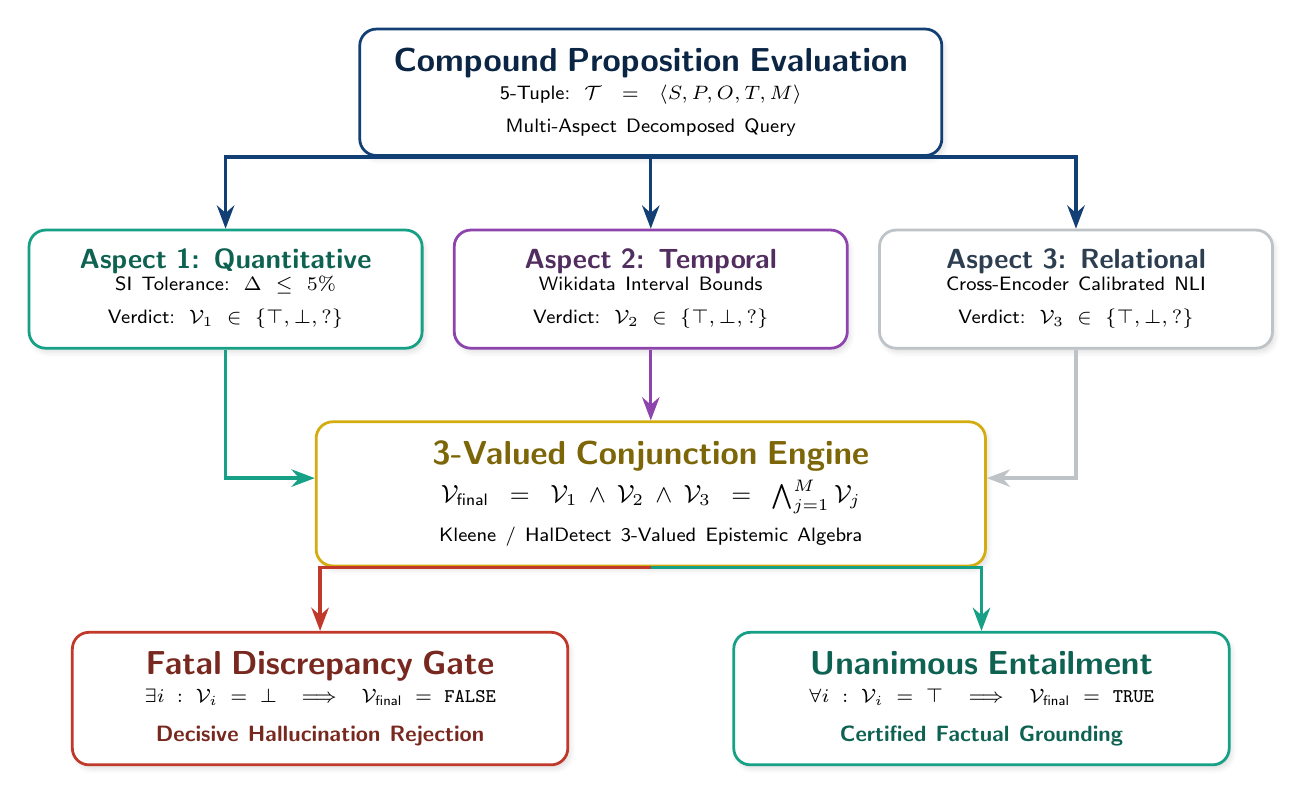
\begin{tikzpicture}[
    font=\sffamily,
    >=Stealth,
    card/.style={
        draw=#1Border, fill=white, line width=1.0pt, rounded corners=6pt,
        blur shadow={shadow blur steps=4, shadow xshift=1pt, shadow yshift=-1.5pt, shadow opacity=12},
        align=center, inner sep=7pt
    },
    wire/.style={
        ->, line width=1.2pt, draw=#1Border
    }
]

\node[card=navy, minimum width=7.2cm, text width=6.9cm] (input) at (0, 4.5) {
    \textbf{\color{navyDark}\large Compound Proposition Evaluation}\\
    \vspace{2pt}
    \scriptsize 5-Tuple: $\mathcal{T} = \langle S, P, O, T, M \rangle$\\
    \scriptsize Multi-Aspect Decomposed Query
};

% 3 Parallel Aspect Evaluators
\node[card=emerald, minimum width=4.8cm, text width=4.5cm] (m1) at (-5.4, 2.0) {
    \textbf{\color{emeraldDark} Aspect 1: Quantitative}\\
    \scriptsize SI Tolerance: $\Delta \le 5\%$\\
    \scriptsize Verdict: $\mathcal{V}_1 \in \{\top, \bot, ?\}$
};

\node[card=purple, minimum width=4.8cm, text width=4.5cm] (m2) at (0, 2.0) {
    \textbf{\color{purpleDark} Aspect 2: Temporal}\\
    \scriptsize Wikidata Interval Bounds\\
    \scriptsize Verdict: $\mathcal{V}_2 \in \{\top, \bot, ?\}$
};

\node[card=slate, minimum width=4.8cm, text width=4.5cm] (m3) at (5.4, 2.0) {
    \textbf{\color{slateDark} Aspect 3: Relational}\\
    \scriptsize Cross-Encoder Calibrated NLI\\
    \scriptsize Verdict: $\mathcal{V}_3 \in \{\top, \bot, ?\}$
};

\draw[wire=navy] (input.south) -| (m1.north);
\draw[wire=navy] (input.south) -- (m2.north);
\draw[wire=navy] (input.south) -| (m3.north);

% 3-Valued Conjunction Engine
\node[card=amber, minimum width=8.5cm, text width=8.0cm] (dag) at (0, -0.6) {
    \textbf{\color{amberDark}\large 3-Valued Conjunction Engine}\\
    \vspace{3pt}
    \small $\mathcal{V}_{\text{final}} = \mathcal{V}_1 \wedge \mathcal{V}_2 \wedge \mathcal{V}_3 = \bigwedge_{j=1}^M \mathcal{V}_j$\\
    \vspace{2pt}
    \scriptsize Kleene / HalDetect 3-Valued Epistemic Algebra
};

\draw[wire=emerald] (m1.south) |- ($(dag.west) + (0, 0.2)$);
\draw[wire=purple] (m2.south) -- (dag.north);
\draw[wire=slate] (m3.south) |- ($(dag.east) + (0, 0.2)$);

% Decision Branches
\node[card=crimson, minimum width=6.2cm, text width=5.8cm] (rule1) at (-4.2, -3.2) {
    \textbf{\color{crimsonDark}\large Fatal Discrepancy Gate}\\
    \vspace{2pt}
    \scriptsize $\exists i: \mathcal{V}_i = \bot \implies \mathcal{V}_{\text{final}} = \textbf{\texttt{FALSE}}$\\
    \vspace{2pt}
    \textbf{\color{crimsonDark}\footnotesize Decisive Hallucination Rejection}
};

\node[card=emerald, minimum width=6.2cm, text width=5.8cm] (rule2) at (4.2, -3.2) {
    \textbf{\color{emeraldDark}\large Unanimous Entailment}\\
    \vspace{2pt}
    \scriptsize $\forall i: \mathcal{V}_i = \top \implies \mathcal{V}_{\text{final}} = \textbf{\texttt{TRUE}}$\\
    \vspace{2pt}
    \textbf{\color{emeraldDark}\footnotesize Certified Factual Grounding}
};

\draw[wire=crimson] (dag.south) -| (rule1.north);
\draw[wire=emerald] (dag.south) -| (rule2.north);

\end{tikzpicture}
\end{document}
